
\documentclass[12pt]{article}
\usepackage[margin=1in]{geometry}
\usepackage{graphicx}
\usepackage{hyperref}
\usepackage{csquotes}
\usepackage[backend=biber,style=authoryear]{biblatex}
\addbibresource{references.bib}
\usepackage{glossaries}

\makeglossaries

% -------- Glossary entries (edit/add as needed) --------
\newglossaryentry{cadre}{
  name={cadre},
  description={A small group of people specially trained for a particular purpose or profession; here, the founding group stewarding family wealth transitions.}
}
\newglossaryentry{founding}{
  name={Founding},
  description={The inaugural gathering that creates the ongoing professional ecosystem supporting family wealth transitions.}
}

\title{LaTeX Export-Ready Templates: Demo Document}
\author{Your Name}
\date{\today}

\begin{document}
\maketitle
\tableofcontents

\section{Introduction}
This minimal project demonstrates export-ready templates:
a bibliography via \texttt{biblatex}/\texttt{biber}, a List of Figures with short captions,
and a \texttt{glossaries} section.

You can cite a book \parencite{chernow1998titan} and an article \parencite{smith2020wealth}.
We use glossary terms like \gls{cadre} and \gls{founding}.

\section{List of Figures}
\listoffigures

\section{Figure Template Usage}
Below is a sample figure included with both a short caption (for the List of Figures) and a longer caption for context.
% ---- Figure template ----
\begin{figure}[h]
  \centering
  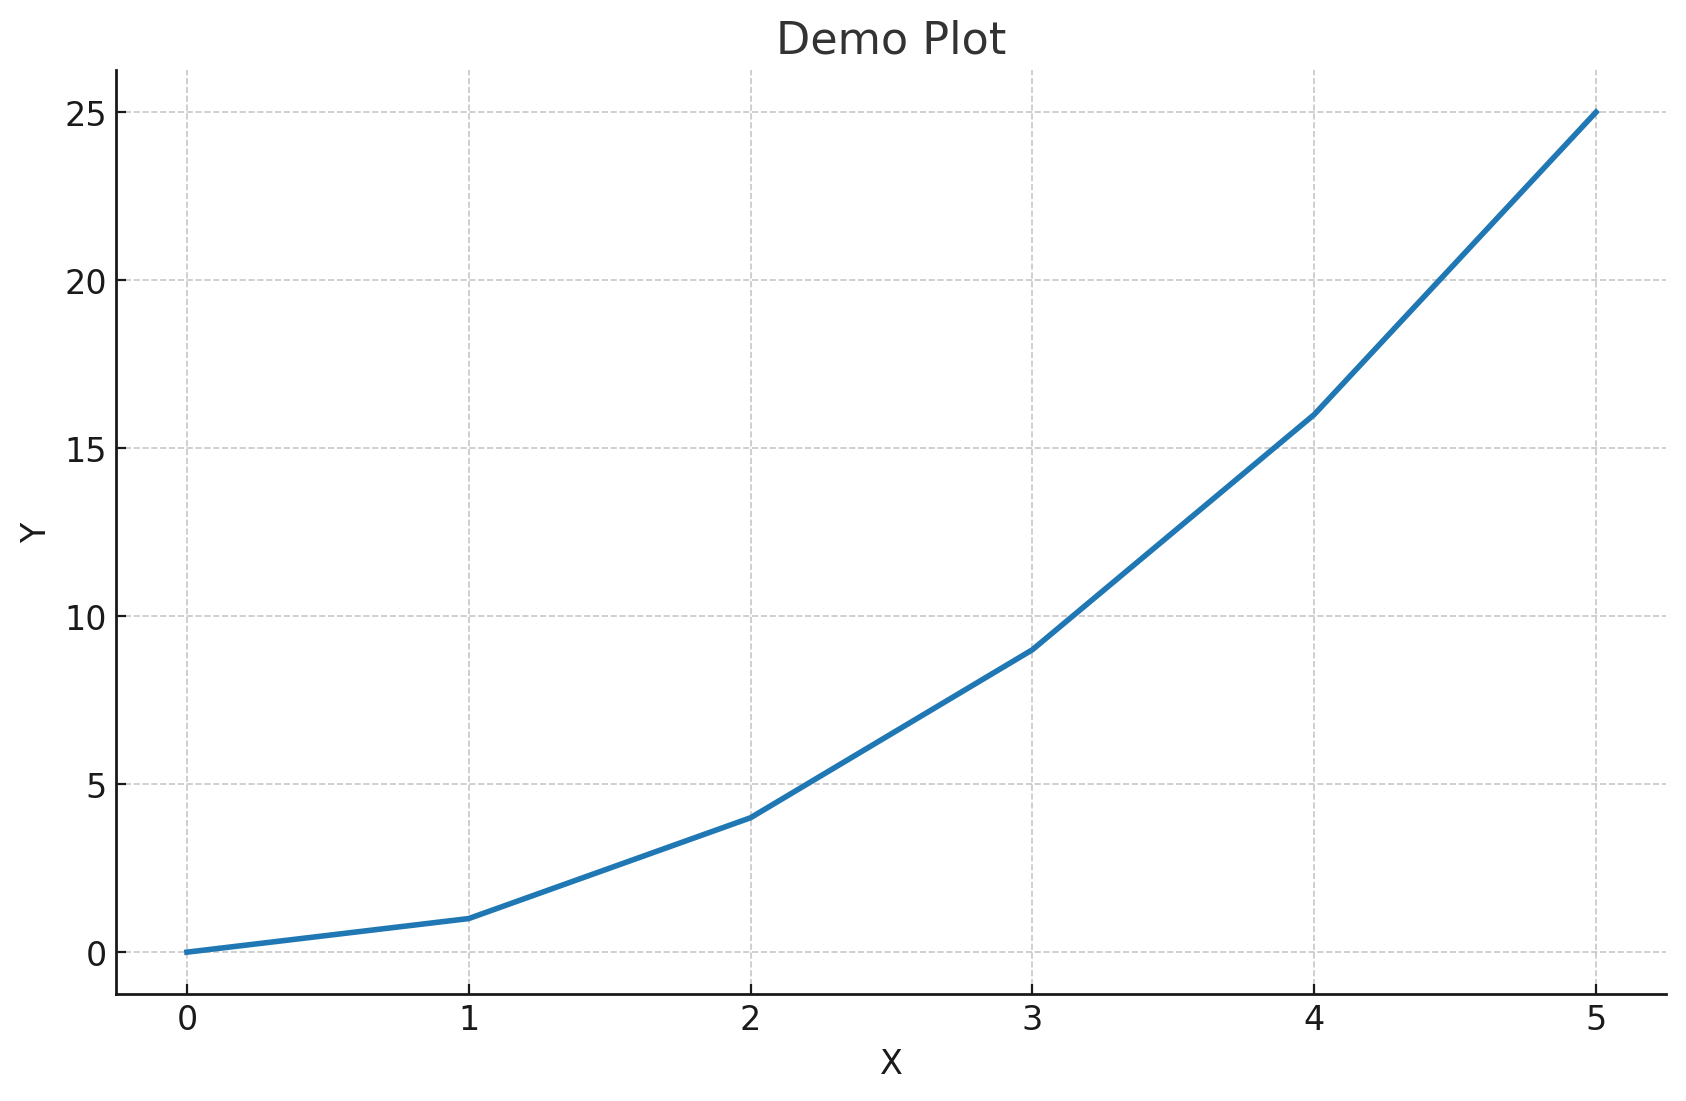
\includegraphics[width=0.7\textwidth]{figure.png}
  \caption[Demo Plot]{Demo Plot --- A simple, generated chart to confirm graphics inclusion, figure captions, and the List of Figures entry.}
  \label{fig:demo}
\end{figure}

\section{Glossary}
% Add all defined entries to the glossary list (optional quality-of-life)
\glsaddall
\printglossaries

\section{References}
\printbibliography

\end{document}
